% ==========================================================================
%  Computational domain and boundary conditions
%
%  Standalone LaTeX document.  On Overleaf: New Project > Blank Project,
%  replace ALL of main.tex with this file (or upload it and set it as the
%  main document) and compile with pdfLaTeX.  In the paper, include the
%  compiled PDF with \includegraphics.
%
%  Generated by make_figures.py; coordinates in mm, origin at the cylinder
%  centre, x downstream, y up.
%  Case: M_inf = 8.03, beta = 18.1 deg -> theta = 12.49 deg, M_2 = 5.252 (gamma = 1.4).
%  R = 38.1 mm, inlet radius 150.39 mm, outlets at phi = +/-65 deg, no-slip wall
%  |phi| <= 45 deg, slip wall beyond, inlet split phi = -12.25 deg.
%  Dashed box: window of fig_typeiv.tex / fig_typeiv_detailed.tex.
% ==========================================================================
\documentclass[border=1pt]{standalone}
% ---- fonts: Helvetica text; sans-serif math (newtxsf) when available
\usepackage[T1]{fontenc}
\usepackage[scaled=0.92]{helvet}
\renewcommand{\familydefault}{\sfdefault}
\IfFileExists{newtxsf.sty}{\usepackage{newtxsf}}{}
\usepackage{tikz}
\usetikzlibrary{arrows.meta}

% ---- colours
\definecolor{ink}{HTML}{111111}
\definecolor{shockgrey}{HTML}{4A4A4A}
\definecolor{dimgrey}{HTML}{808080}
\definecolor{leadergrey}{HTML}{9A9A9A}
\definecolor{bodygrey}{HTML}{E4E4E4}
\definecolor{freeblue}{HTML}{1A5FA8}
\definecolor{postgreen}{HTML}{0E8A62}
\definecolor{slipochre}{HTML}{B06A10}
\definecolor{jetfill}{HTML}{FBEBD3}
\definecolor{zoomred}{HTML}{C0392B}

% ---- styles
\tikzset{
  lbl/.style={font=\sffamily\small, text=ink, inner sep=1.2pt, align=center},
  sml/.style={font=\sffamily\footnotesize, text=ink, inner sep=1.2pt, align=center},
  region/.style={font=\sffamily\small, text=dimgrey, inner sep=1pt},
  leader/.style={draw=leadergrey, line width=0.4pt},
  freeinlet/.style={draw=freeblue, line width=1.5pt},
  postinlet/.style={draw=postgreen, line width=1.5pt},
  outlet/.style={draw=dimgrey, line width=1.1pt, dash pattern=on 3.2pt off 2pt, line cap=butt},
  noslip/.style={draw=ink, line width=1.7pt},
  slip/.style={draw=slipochre, line width=1.7pt, dash pattern=on 2pt off 1.1pt, line cap=butt},
  shockA/.style={draw=shockgrey, line width=0.7pt},
  shockB/.style={draw=ink, line width=1.1pt},
  jetshock/.style={draw=ink, line width=1.1pt},
  shear/.style={draw=ink, line width=0.7pt, dash pattern=on 2.4pt off 1.4pt, line cap=butt},
  cellshock/.style={draw=ink, line width=0.45pt},
  fan/.style={draw=ink, line width=0.45pt, dash pattern=on 1.4pt off 0.9pt, line cap=butt},
  hatch/.style={draw=dimgrey, line width=0.35pt, line cap=butt},
  flow/.style={line width=0.9pt, -{Stealth[length=2.4mm, width=1.8mm]}},
  jetflow/.style={draw=ink, line width=0.75pt, -{Stealth[length=2mm, width=1.5mm]}},
  dim/.style={draw=dimgrey, line width=0.45pt,
              {Stealth[length=1.6mm, width=1.1mm]}-{Stealth[length=1.6mm, width=1.1mm]}},
  triple/.style={circle, fill=ink, inner sep=0pt, minimum size=1.6mm},
  dot/.style={circle, fill=leadergrey, inner sep=0pt, minimum size=1mm},
  panel/.style={font=\sffamily\bfseries\small, inner sep=0pt},
  % grid
  gridline/.style={draw=ink, line width=0.12pt},
  gridedge/.style={draw=ink, line width=0.6pt},
  axis/.style={draw=ink, line width=0.5pt},
  tick/.style={draw=ink, line width=0.4pt},
  ticklbl/.style={font=\sffamily\footnotesize, text=ink, inner sep=1.5pt},
  zoombox/.style={draw=zoomred, line width=0.6pt},
}
% panel letter: change to \newcommand{\panellabel}{} to remove it
\newcommand{\panellabel}{(a)}

\begin{document}
\sffamily\small
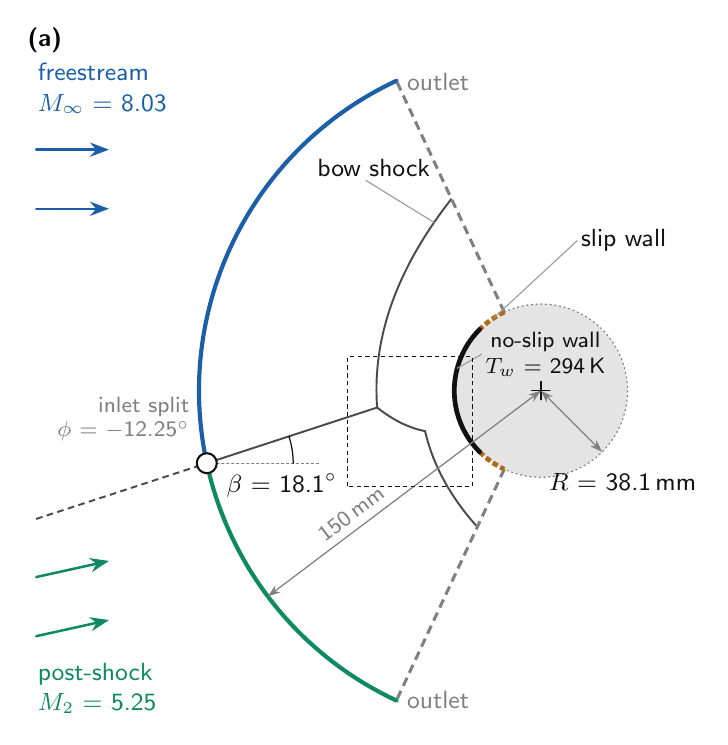
\begin{tikzpicture}[x=1mm, y=1mm, line cap=round, line join=round]

\begin{scope}[shift={(65.25,44.18)}, x=0.28873mm, y=0.28873mm]

  % cylinder (dotted where it lies outside the domain)
  \fill[bodygrey] (0,0) circle[radius=38.1];
  \draw[dimgrey, line width=0.45pt, dash pattern=on 0.4pt off 1.3pt]
    (115:38.1) arc[start angle=115, end angle=-115, radius=38.1];

  % shock system (no-field solution), clipped to the domain
  \begin{scope}
    \clip (115:150.387) arc[start angle=115, end angle=245, radius=150.387] -- (245:38.1)
      arc[start angle=245, end angle=115, radius=38.1] -- cycle;
    \draw[shockA]
      (-72.03,-7.42) -- (-72.19,-4.94) -- (-72.29,-2.46) -- (-72.33,0.02) -- (-72.31,2.51) --
      (-72.24,4.99) -- (-72.1,7.47) -- (-71.91,9.95) -- (-71.66,12.43) -- (-71.36,14.91) --
      (-70.99,17.39) -- (-70.57,19.87) -- (-70.09,22.35) -- (-69.55,24.83) --
      (-68.96,27.31) -- (-68.3,29.79) -- (-67.59,32.28) -- (-66.82,34.76) -- (-66,37.24) --
      (-65.11,39.72) -- (-64.17,42.2) -- (-63.17,44.68) -- (-62.11,47.16) --
      (-60.99,49.64) -- (-59.82,52.12) -- (-58.59,54.6) -- (-57.3,57.08) -- (-55.96,59.56) --
      (-54.55,62.05) -- (-53.09,64.53) -- (-51.57,67.01) -- (-50,69.49) -- (-48.36,71.97) --
      (-46.67,74.45) -- (-44.93,76.93) -- (-43.12,79.41) -- (-41.26,81.89) --
      (-39.34,84.37) -- (-37.37,86.85) -- (-35.33,89.33) -- (-33.24,91.82) -- (-31.1,94.3) --
      (-28.89,96.78) -- (-26.63,99.26) -- (-24.31,101.74) -- (-21.94,104.22) --
      (-19.51,106.7) -- (-17.02,109.18) -- (-14.48,111.66) -- (-11.88,114.14) --
      (-9.22,116.62) -- (-6.51,119.1) -- (-3.74,121.59) -- (-0.91,124.07) -- (1.97,126.55) --
      (4.91,129.03) -- (7.9,131.51) -- (10.95,133.99) -- (14.05,136.47) -- (17.22,138.95) --
      (20.43,141.43) -- (23.7,143.91) -- (27.03,146.39) -- (30.42,148.87) --
      (33.85,151.36) -- (37.35,153.84) -- (40.9,156.32) -- (44.5,158.8) -- (48.16,161.28) --
      (51.87,163.76) -- (53.75,165);
    \draw[shockA]
      (-50.94,-17.8) -- (-50.36,-20.16) -- (-49.71,-22.5) -- (-48.98,-24.82) --
      (-48.19,-27.13) -- (-47.33,-29.43) -- (-46.39,-31.7) -- (-45.39,-33.97) --
      (-44.32,-36.22) -- (-43.18,-38.45) -- (-41.97,-40.67) -- (-40.69,-42.87) --
      (-39.34,-45.05) -- (-37.92,-47.23) -- (-36.44,-49.38) -- (-34.88,-51.52) --
      (-33.26,-53.65) -- (-31.56,-55.76) -- (-29.8,-57.85) -- (-27.97,-59.93) --
      (-26.07,-62) -- (-24.1,-64.05) -- (-22.06,-66.08) -- (-19.96,-68.1) --
      (-17.79,-70.1) -- (-15.55,-72.09) -- (-13.24,-74.07) -- (-10.86,-76.02) --
      (-8.42,-77.97) -- (-5.91,-79.9) -- (-3.33,-81.81) -- (-0.69,-83.71) -- (2.02,-85.6) --
      (4.79,-87.47) -- (7.64,-89.32) -- (10.54,-91.17) -- (13.52,-92.99) -- (16.56,-94.8) --
      (19.66,-96.6) -- (22.83,-98.38) -- (26.06,-100.15) -- (29.36,-101.91) --
      (32.73,-103.65) -- (36.15,-105.37) -- (39.64,-107.09) -- (43.2,-108.78) --
      (46.82,-110.47) -- (50.5,-112.14) -- (54.24,-113.79) -- (58.05,-115.44) --
      (61.91,-117.07) -- (65.84,-118.68) -- (69.83,-120.28) -- (73.89,-121.87) --
      (78,-123.44) -- (82.18,-125) -- (86.41,-126.55) -- (90.71,-128.08) --
      (95.06,-129.61) -- (99.48,-131.11) -- (103.95,-132.61) -- (108.48,-134.09) --
      (113.07,-135.56) -- (117.72,-137.01) -- (122.43,-138.45) -- (127.2,-139.88) --
      (132.02,-141.3) -- (136.9,-142.71) -- (141.84,-144.1) -- (146.83,-145.48) --
      (149.35,-146.16);
    \draw[shockA]
      (-72.03,-7.42) -- (-70.95,-8.26) -- (-69.87,-9.06) -- (-68.79,-9.84) --
      (-67.71,-10.58) -- (-66.62,-11.29) -- (-65.54,-11.96) -- (-64.46,-12.6) --
      (-63.38,-13.21) -- (-62.3,-13.78) -- (-61.22,-14.32) -- (-60.14,-14.83) --
      (-59.05,-15.3) -- (-57.97,-15.74) -- (-56.89,-16.15) -- (-55.81,-16.53) --
      (-54.73,-16.87) -- (-53.65,-17.18) -- (-52.56,-17.45) -- (-51.48,-17.69) --
      (-50.94,-17.8);
    \draw[shockA] (-146.96,-31.91) -- (-72.03,-7.42);
  \end{scope}
  \draw[shockA, dash pattern=on 2.4pt off 1.6pt, line cap=butt] (-222,-56.43) -- (-146.96,-31.91);

  % boundaries
  \draw[freeinlet] (192.25:150.387) arc[start angle=192.25, end angle=115, radius=150.387];
  \draw[postinlet] (245:150.387) arc[start angle=245, end angle=192.25, radius=150.387];
  \draw[outlet] (115:38.1) -- (115:150.387);
  \draw[outlet] (245:38.1) -- (245:150.387);
  \draw[slip]   (115:38.1) arc[start angle=115, end angle=135, radius=38.1];
  \draw[slip]   (225:38.1) arc[start angle=225, end angle=245, radius=38.1];
  \draw[noslip] (135:38.1) arc[start angle=135, end angle=225, radius=38.1];
  \draw[ink, line width=0.5pt] (-4,0) -- (4,0) (0,-4) -- (0,4);

  % inlet split and imposed shock angle
  \draw[dimgrey, line width=0.4pt, dash pattern=on 0.8pt off 1pt] (-146.96,-31.91) -- ++(50,0);
  \draw[ink, line width=0.45pt] (-108.96,-31.91) arc[start angle=0, end angle=18.1, radius=38];
  \node[lbl, anchor=north west] at (-139.96,-34.91) {$\beta$ = 18.1$^\circ$};
  \filldraw[fill=white, draw=ink, line width=0.75pt] (-146.96,-31.91) circle[radius=4.4];
  \node[sml, text=dimgrey, anchor=south east, align=right] at (-152.96,-23.91)
    {inlet split\\[-0.2ex]$\phi$ = $-$12.25$^\circ$};

  % inflow
  \foreach \yy in {106, 80} {\draw[flow, freeblue] (-222,\yy) -- ++(32,0);}
  \foreach \yy in {-82, -108} {\draw[flow, postgreen] (-222,\yy) -- ++(12.49:32.8);}
  \node[lbl, text=freeblue, anchor=south west, align=left] at (-223,120)
    {freestream\\$M_\infty$ = 8.03};
  \node[lbl, text=postgreen, anchor=north west, align=left] at (-223,-118)
    {post-shock\\$M_2$ = 5.25};

  % boundary labels
  \node[sml] (ns) at (2,16) {no-slip wall\\$T_w$ = 294\,K};
  \draw[leader] (ns.west) -- (-36.8,9.86);
  \node[lbl, anchor=west] (sw) at (16,66) {slip wall};
  \draw[leader] (sw.west) -- (-20.75,31.95);
  \node[lbl, text=dimgrey, anchor=south west] at (-60.56,130.3) {outlet};
  \node[lbl, text=dimgrey, anchor=north west] at (-60.56,-130.3) {outlet};
  \node[lbl, anchor=west] (bs) at (-100,98) {bow shock};
  \draw[leader] ([xshift=-1mm]bs.south) -- (-46.99,74);

  % dimensions
  \draw[dim] (0,0) -- (-45:38.1);
  \node[lbl, anchor=north] at (35.94,-34.94) {$R$ = 38.1\,mm};
  \draw[dim] (0,0) -- (217:150.387);
  \node[sml, text=dimgrey, rotate=37.00] at (-83.48,-54.14) {150\,mm};

  % close-up window (other figure)
  \draw[ink, line width=0.45pt, dash pattern=on 1.6pt off 1.2pt, line cap=butt]
    (-85,-42) rectangle (-30,15);
\end{scope}

% panel letter
\node[panel, anchor=north west] at (0,90.35) {\panellabel};
\end{tikzpicture}
\end{document}
